\chapter{Investimento Ótimo}
\localtableofcontents 

Este capítulo é baseado nas notas de aula do curso, ministrado em 11/08/2023 e 14/08/2023, e nos capítulos 21 e 22 de \textcite{cretì_fontini_2019}.

A análise deste capítulo é parecida com a dos exercícios de Despacho Ótimo dos capítulos anteriores. Entretanto, flexibilizamos uma hipótese que anteriormente era imposta: capacidade máxima de geração fixa. O propósito deste capítulo é pensar em formas de determinação endógena dessa capacidade.

\section{Problema Centralizado de Investimento Ótimo}
Suponha a existência de uma única tecnologia de geração i.e. todas as usinas possuem o mesmo custo de produção. A maximização deste problema no instante $t$ é dada por:
\begin{align*}
    \max_{M_i^{max},q_i,q^d}&\quad U(q^d) - \sum_{i=1}^nc_i(q_i,M_i^{max})\\
    \textbf{s.a.}&\quad q^d=\sum_iq_i\\
    &\quad q_i\ge0,\forall i\\
    &\quad q_i\le M_i^{max},\forall i
\end{align*}
Implicando o Lagrangiano:
\begin{align*}
    \mathcal{L}=\sum_{i=1}^nc_i(q_i,M_i^{max})-U(q^d)+\mu\left(\sum_iq_i-q^d\right)-\sum_i\lambda_iq_i+\sum_i\lambda_{n+i}(q_i-M_i^{max})
\end{align*}
Implicando as CPOs:
\begin{align*}
    \frac{\partial\mathcal{L}}{\partial q_i}&=c_{i,q_i}+\mu-\lambda_i+\lambda_{n+i}=0\Longleftrightarrow c_{i,q_i} =-\mu-\lambda_{n+i}-\lambda_i,\forall i \\
    \frac{\partial\mathcal{L}}{\partial q^d}&=-U'(q^d)-\mu=0 \Longleftrightarrow  U'(q^d) = -\mu\\
    \frac{\partial\mathcal{L}}{\partial M_i^{max}}&=c_{i,M_i^{max}}-\lambda_{n+i}=0 \Longleftrightarrow c_{i,M_i^{max}}=\lambda_{n+i}, \forall i
\end{align*}
Onde os subscritos em $c_i$ denotam as derivadas parciais. Considerando a solução interna teremos:
\begin{align*}
    \lambda_{n+i}&=c_{i,M_i^{max}},\forall i\\
    \lambda_{n+i}&=(U'(q^d)-c_{i,q_i})\cdot\mathbbm{1}[M_i^{max}=q_i],\forall i
\end{align*}
Igualando as equações e dividindo pelo horizonte de tempo $T$ temos:
\begin{align*}
    \underbrace{\frac{c_{i,M_i^{max}}}{T}}_{hRC_i} = (\underbrace{U'(q^d)}_{VOLL}-\underbrace{c_{i,q_i}}_{c_i})\cdot\underbrace{\frac{\mathbbm{1}[M_i^{max}=q_i]}{T}}_{P(q^d>M_i^{max})\equiv LOLP_i},\forall i
\end{align*}
Onde $hRC_i$ é o custo do aluguel do capital instalado na usina $i$ e VOLL e LOLP são conceitos definidos no Capítulo~3. Ora, então temos que LOLP pode ser definido também (no longo prazo) como:
\begin{align*}
    LOLP_i = \frac{hRC_i}{VOLL-c_i}
\end{align*}
Assim, vemos como é possível definir o nível ótimo de capacidade: A capacidade ótima de longo prazo é aquela que faz LOLP atender à equação acima. Mais ainda, note que $c_i$ é de uma ordem de magnitude muito inferior a $VOLL$ e, portanto, podemos ignorá-la de forma a obter:
\begin{align*}
    LOLP_i\approx \frac{YRC_i}{VOLL}
\end{align*}
Onde $YRC_i$ denota o aluguel anual do capital instalado na usina $i$. A equação acima é normalmente referida como "preço da carga máxima" ou \textit{VOLL-pricing}.

\section{Problema Descentralizado de Investimento Ótimo}
No problema descentralizado o objetivo da firma é maximizar seus lucros. Iremos supor 3 tecnologias, de forma a termos usinas de "carga base", "carga de pico" e \textit{mid-merit}. Mais ainda, note que o preço do produto final dependerá das decisões de produção de todas as firmas conjuntamente.

Vamos começar pelo problema da firma de carga de pico (\textit{peaker}). Note que ela só produz quando $q^d>M_1^{max}+M_2^{max}$, por definição. Mais ainda, essa firma se depara com dois cenários de preços: 1) há desligamento de carga e, portanto, o preço é $\phi=VOLL$, o que ocorre com probabilidade $v_L=LOLP$; e 2) ela é a firma marginal e o preço será o do sistema i.e. $c_3$, ocorrendo com probabilidade $cf_3-v_L$. A receita do 
\textit{peaker} é dada, então, por:
\[\pi_3=\phi v_LM_3^{max}+c_3(cf_3-v_L)M_3^{max}\]
Seus custos dados por:
\[YRC_3M_3^{max}+c_3cf_3M_3^{max}\]
Implicando lucro:
\[\pi_3=(\phi-c_3) v_LM_3^{max}-YRC_3M_3^{max}\]
Analogamente, teremos que os lucros das firmas \textit{mid-merit} e "carga base" (\textit{baseload}) serão dados por, respectivamente:
\begin{align*}
    \pi_2&=(\phi-c_3)v_LM_2^{max}+(c_3-c_2)cf_3M_2^{max}-YRC_2M_2^{max}\\
    \pi_1&=(\phi-c_3)v_LM_1^{max}+(c_3-c_2)cf_3M_1^{max}+(c_2-c_1)cf_2M_1^{max}-YRC_1M_1^{max}
\end{align*}
É imediato perceber que as CPOs do problema individual de cada firma (onde elas maximizam seu respectivo $M_i^{max}$) implicam:
\begin{align*}
    YRC_3&=(\phi-c_3)v_L\\
    YRC_2&=(\phi-c_3)v_L+(c_3-c_2)cf_3\\
    YRC_1&=(\phi-c_3)v_L+(c_3-c_2)cf_3+(c_2-c_1)cf_2
\end{align*}
Tal qual esperado, esses valores são idênticos aos encontrados no problema de minimização de custos (veja Cap. 21 de  \textcite{cretì_fontini_2019}), ou seja, mais uma aplicação do Primeiro Teorema do Bem-Estar - o que é esperado vide a falta de fricções de mercado. A segunda conclusão que temos deste resultado é que, em perfeita concorrência, há lucro econômico 0 ($\pi_i=0,\forall i$) i.e. os investidores perfeitamente repagam seus investimentos.

\section{Mecanismos de Remuneração de Capacidade (CRMs)}
Uma discussão do mundo real relacionada à esse tópico é que os retorno do capital investido no setor de eletricidade (não confundir com lucro econômico) são muito baixos e, portanto, existem poucos incentivos à atores privados investirem o suficiente para chegar-se aos níveis ótimos. Como os Operadores do Sistema prezam pela eficiência do sistema, algum mecanismo para aumentar esses incentivos deve ser criado.

A fins de comparação, considere apenas duas firmas seguindo a lógica do exercício da sessão anterior (\textit{first-best} i.e. mercados perfeitos):
\begin{align*}
    YRC_2&=(\phi-c_2)v_L\\
    YRC_1&=(\phi-c_2)v_L+(c_2-c_1)cf_2
\end{align*}
Abaixo segue um exemplo desses mecanismos. Para uma discussão mais aprofundada veja o Capítulo~22 de \textcite{cretì_fontini_2019}.

\subsection{Teto de Preços}
Se tivermos um teto de preços $\overline{p}$, será possível chegar à alocação ótima de investimentos se eles forem remunerados ao nível ótimo. Suponha um sistema com limitações de capacidade i.e. $M_2^{mis}=M_2^*-M_2^{ins}$, onde $=M_2^*$ é a capacidade ótima, $M_2^{ins}$ a capacidade instalada e $M_2^{mis}$ a capacidade faltante. 

Por causa da falta de capacidade, temos que $v_L^{ins}>v_L^*$. Mais ainda, a existência dessa falta de capacidade é o teto de preços baixo demais i.e. $\overline{p}<\phi$. Repare a mudança na estrutura de lucros implica duas CPOs marginalmente diferentes:
\begin{align*}
    \text{sem teto de preços:}&\quad YRC_2=(\phi-c_2)v_L^*\\
    \text{com teto de preços:}&\quad YRC_2=(\overline{p}-c_2)v_L^{ins}
\end{align*}
Graficamente, essa dinâmica pode ser observada na Figura~\ref{fig:price_cap}. A área tracejada denota a perda de receitas decorrentes do teto de preços, enquanto a área sombreada denota o ganho de receitas decorrentes do teto. Note que:
\begin{figure}
    \centering
    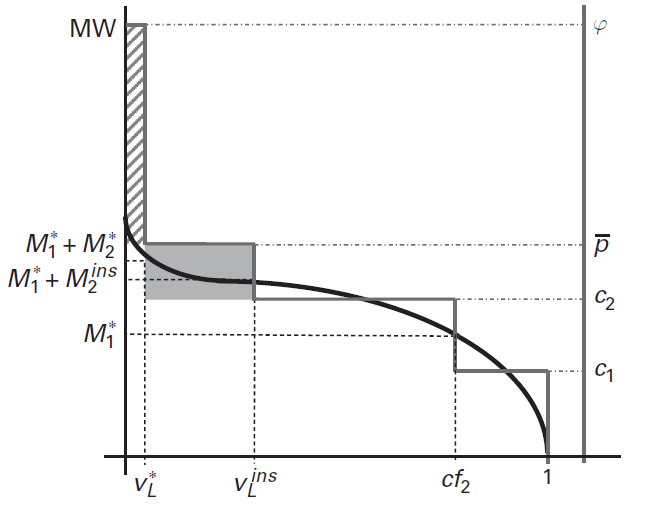
\includegraphics[scale=.4]{figure/price_cap.png}
    \caption{Efeito de Teto de Preços}
    \label{fig:price_cap}
\end{figure}
\begin{align*}
    \underbrace{(\overline{p}-c_2)\cdot(v_L^{ins}-v_L^*)}_{\text{ganhos}} - \underbrace{(\phi-\overline{p})\cdot v_L^*}_{\text{perdas}} <0
\end{align*}
pois, caso contrário, o nível de investimentos seria $M_2^{ins}\ge M_2^*$. Assuma, agora, que o operador paga $k$ por unidade de capital instalado. Com a CRM, o lucro líquido da usina 2 fica:
\begin{align*}
    \overline{\pi_2} =(\overline{p}-c_2)v_L^{ins}M_2^{ins} + kM_2^{ins} - YRC_2M_2^{ins}
\end{align*}
Resta perguntar, então, qual o nível $k$ que maximiza o bem-estar. Ora, é fácil intuir que se remunerarmos a firma pela sua perda de receitas decorrente do teto de preços, a alocação será a ótima. Analiticamente, seja $k = (\phi-\overline{p}) v_L^*-(\overline{p}-c_2)(v_L^{ins}-v_L^*)$. Temos então que:
\begin{align*}
    \overline{\pi_2}(M_2^{ins}) &=(\overline{p}-c_2)v_L^{ins}M_2^{ins} + [(\phi-\overline{p}) v_L^*-(\overline{p}-c_2)(v_L^{ins}-v_L^*)]M_2^{ins} - YRC_2M_2^{ins}\\
    &=(\phi-\overline{p}) v_L^*M_2^{ins} - YRC_2M_2^{ins}\\
    &=\pi^*(M_2^{ins})
\end{align*}
Note que, maximizando em $M_2^{ins}$, o resultado da otimização de lucro levará à mesma alocação de capacidade do ótimo i.e. na ausência de teto de preços. Considerações sobre a firma \textit{baseload} podem ser vistas no Capítulo~22 de \textcite{cretì_fontini_2019}.